\documentclass{article}
\usepackage[left=2cm, right=2cm, top=3cm, bottom=3cm]{geometry}
\usepackage[utf8]{inputenc}
\usepackage{amsmath}
\usepackage{amsthm}
\usepackage{amssymb}
\usepackage{hyperref}
\usepackage{graphicx}

\hypersetup{
    colorlinks,
    citecolor=black,
    filecolor=black,
    linkcolor=black,
    urlcolor=black
}

\newcommand{\R}{\mathbb{R}}
\newcommand{\Rext}{\widetilde{\mathbb{R}}}

\newenvironment{mytheorem}[1]
{\begin{theorem}[#1]\setlength{\leftskip}{2cm}}
{\end{theorem}}

\title{Teoria Analisi 1}

\begin{document}
\maketitle
\tableofcontents\newpage

\begin{flushleft}

\section{Teorema del differenziale (Lagrange - Rolle generalizzato) - Solo enunciato}
{2.2em}$f: I \subset \R, I$ intervallo, $x_0 \in I$, $x_0$ interno ad $I$, $f$ derivabile in $x_0$.
\\Allora: $\exists$ w: I $\rightarrow \R$ t.c. w è continua in $x_0$, w($x_0$) = 0 e
\[
    f(x_0) + f'(x_0)(x-x_0)+w(x)(x-x_0)
\]
\\dove: $f(x_0) + f'(x_0)(x-x_0)$ è la tangente
\\\hspace{2.3em} $w(x)(x-x_0)$ è l'errore causato da alcuni fattori, \underline{lo possiamo trascurare.}


\section{Teorema dell'unicità del limite}
\subsection{Enunciato}
$f: A \subset \R \rightarrow \R$, $x_0 \in \Rext$ punto di accumulazione per $A$
Se:
\begin{enumerate}
    \item $\lim_{x \to x_0} f(x) = l_1 \in \Rext$
    \item $\lim_{x \to x_0} f(x) = l_2 \in \Rext$
\end{enumerate}
Allora: $\mathbf{l_1 = l_2}$

\subsection{Dimostrazione}

\begin{enumerate}
    \item[ip1)] $\forall V l_1 $ intorno di $l_1 \exists U x_0$ intorno di $x_0$ t.c. $f(x)\in\forall l_1 $ per ogni $x\in (U x_0 \bigcap A) - \{0\}$
    \item[ip2)] $\forall V l_2 $ intorno di $l_2 \exists U' x_0$ intorno di $x_0$ t.c. $f(x)\in\forall l_2 $ per ogni $x\in (U' x_0 \bigcap A) - \{0\}$
\end{enumerate}

\begin{figure}[h]
    \centering
    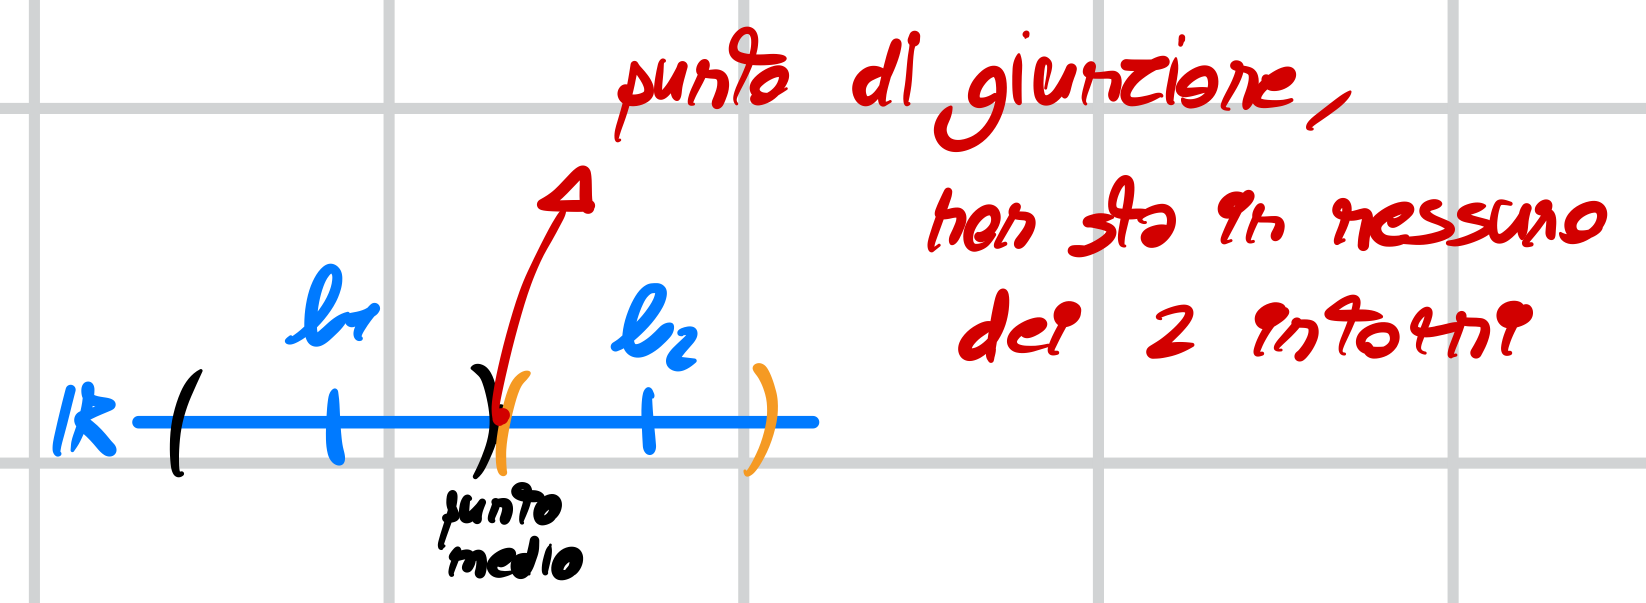
\includegraphics[width=10em]{./images/unicitaLimite.PNG}
\end{figure}

Per contraddizione: $l_1 \neq l_2$
\\Allora $\exists Vl_1, Vl_2$ intorni di $l_1$ e $l_2$ (rispettivamente) tali che: $Vl_1 \bigcup Vl_2 \neq \emptyset$
\\$Wx_0 = \bigcup U'x_0$ è un intorno di $x_0$
\\Sia $x \in(Wx_0 \bigcup A) - \{x_0\} \neq \emptyset$ (perché $x_0$ è di accumulazione)

\begin{align*}
    \Rightarrow
    \begin{cases}
        f(x) \in Vl_1 \\
        z = x^2 - 3
    \end{cases}
\end{align*}


\section{Teorema fondamentale del calcolo integrale (TFCI)}
 $[a,b] \subset \R$, $a < b$. $f$ R-integrale su $[a,b]$.
 $\exists x_1 \in [a,b]$ t.c. $f$ sia continua in $x_1$.

\section{Teorema del porcodio}
porcodio
\end{flushleft}
\end{document}